\documentclass[aspectratio=169,11pt]{beamer}
\usepackage[utf8]{inputenc}
\usepackage[T1]{fontenc}
\usepackage[spanish]{babel}
\usepackage{amsmath,amssymb}
\usepackage{tikz}
\usetikzlibrary{arrows.meta,angles,calc,positioning}
\usetheme{Madrid}
\usecolortheme{default}
\setbeamertemplate{navigation symbols}{}
\setbeamertemplate{blocks}[rounded][shadow=false]
\newcommand{\ang}[1]{\angle #1^\circ}

\title[Decibelios y Bode]{Paso 4: Decibelios y escala logarítmica}
\subtitle{Convertir productos en sumas para dibujar $P(j\omega)$ a mano}
\author{Curso de control robusto (QFT)}
\date{}
\begin{document}
\begin{frame}\titlepage\end{frame}

\begin{frame}{Dónde encaja este paso}
  \tiny
  \begin{enumerate}\setlength{\itemsep}{-2pt}
    \item[1.] Números complejos \hfill \textcolor{gray}{(hecho)}
    \item[2.] Funciones de transferencia: $s$, polos y ceros \hfill \textcolor{gray}{(hecho)}
    \item[3.] Respuesta en frecuencia: $s=j\omega$, magnitud y fase \hfill \textcolor{gray}{(hecho)}
    \item[\textbf{4.}] \textbf{Decibelios y escala logarítmica (Bode)} \hfill $\leftarrow$ estamos aquí
    \item[5.] Realimentación: $L$, $T=\frac{L}{1+L}$, $S=\frac{1}{1+L}$
    \item[6.] Nichols chart
    \item[7.] Incertidumbre y templates
    \item[8.] Especificaciones $\rightarrow$ bounds
    \item[9.] Loop shaping, prefiltro y verificación
    \item[10.] QFT en control digital
    \item[11.] Dos caminos digitales: $z$ y $w$
    \item[12.] Estabilidad, límites, más especificaciones y caso real
    \item[13.] Muestreo por eventos con periodo base $T$
    \item[14.] Sistemas de dos estados: lazo interno y externo
    \item[15.] QFT y sistemas no lineales
    \item[16.] Algoritmos de QFT: cómo funcionan por dentro
    \item[17.] QFT en Python: una biblioteca paso a paso
    \item[18.] QFT en MATLAB: el mismo código, otra sintaxis
    \item[19.] Historia, panorama y bibliografía
  \end{enumerate}
  \vspace{4pt}
  \begin{block}{Objetivo de hoy}
    Entender por qué se usan los decibelios, y dibujar el Bode de cualquier $P$ \textbf{sumando} las curvas de sus factores. Esa idea de ``sumar'' es la que hará útil el Nichols chart.
  \end{block}
\end{frame}

\begin{frame}{Los decibelios: una tabla que conviene saberse}
  \small
  \begin{columns}[T]
  \begin{column}{0.48\textwidth}
    \[ |P|_{\text{dB}}=20\log_{10}|P| \]
    \centering
    \begin{tabular}{r|r}
      $|P|$ & dB\\ \hline
      $0.1$ & $-20$\\
      $0.5$ & $-6.02$\\
      $1/\sqrt2=0.707$ & $-3.01$\\
      $1$ & $0$\\
      $\sqrt2=1.414$ & $3.01$\\
      $2$ & $6.02$\\
      $10$ & $20$\\
      $100$ & $40$
    \end{tabular}
  \end{column}
  \begin{column}{0.5\textwidth}
    \begin{block}{Dos reglas de bolsillo}
      \begin{itemize}
        \item $\times10$ en magnitud $=$ $+20$ dB.
        \item $\times2$ en magnitud $\approx$ $+6$ dB.
      \end{itemize}
    \end{block}
    \begin{block}{Qué significa 0 dB}
      $|P|=1$: la salida tiene la misma amplitud que la entrada. Por encima de 0 dB amplifica, por debajo atenúa.
    \end{block}
    \begin{alertblock}{Ojo}
      Es 20 y no 10 porque $|P|$ es una \emph{amplitud}; el 10 se usa para potencias.
    \end{alertblock}
  \end{column}
  \end{columns}
\end{frame}

\begin{frame}{Por qué dB: un producto se convierte en una suma}
  \small
  Si $P(s)=K\cdot F_1(s)\cdot F_2(s)\cdots$, en $s=j\omega$ los complejos se multiplican (paso 1):
  \[ |P|=|K|\,|F_1|\,|F_2|\cdots \qquad \angle P=\angle K+\angle F_1+\angle F_2+\cdots \]
  Tomando $20\log_{10}$ del módulo, el producto pasa a ser una suma:
  \[ \boxed{\;|P|_{\text{dB}}=|K|_{\text{dB}}+|F_1|_{\text{dB}}+|F_2|_{\text{dB}}+\cdots\;} \]
  \begin{block}{Consecuencia práctica}
    La curva de $P$ en dB (y la de su fase) es la \textbf{suma} de las curvas de cada factor. Basta saber dibujar cuatro tipos de factor.
  \end{block}
  \begin{alertblock}{Esto vuelve a importar}
    En QFT $L=G\cdot P$ (controlador por planta). En dB, \emph{añadir un controlador es sumar su curva}. Por eso se dibuja todo en dB y en grados.
  \end{alertblock}
\end{frame}

\begin{frame}{Los cuatro bloques elementales}
  \footnotesize
  \centering
  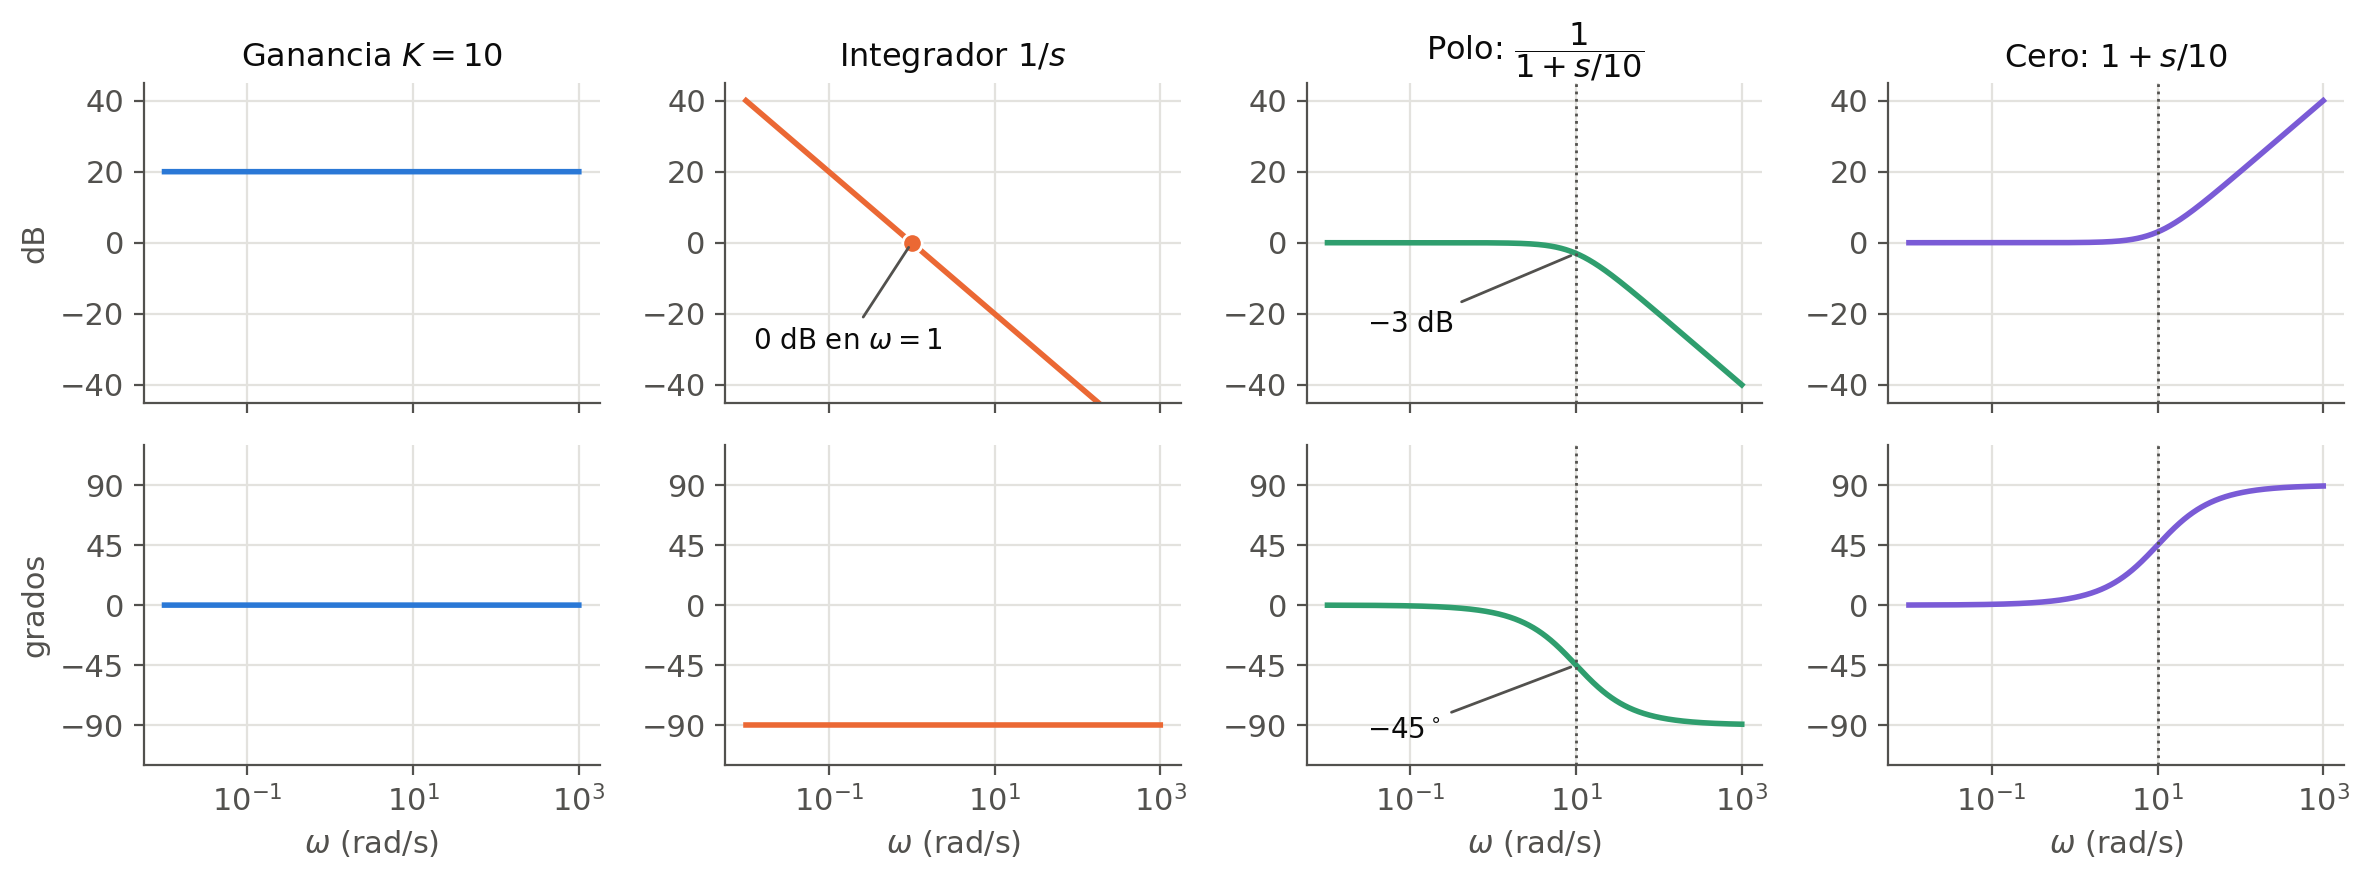
\includegraphics[width=\textwidth]{fig/bloques.png}\\[2pt]
  \begin{tabular}{p{0.19\textwidth}p{0.21\textwidth}p{0.23\textwidth}p{0.23\textwidth}}
    \textbf{Ganancia:} recta horizontal a $20\log_{10}K$; fase $0^\circ$ (o $\pm180^\circ$ si $K<0$)
    & \textbf{Integrador:} $-20$ dB/dec, pasa por 0 dB en $\omega=1$; fase $-90^\circ$
    & \textbf{Polo en $a$:} plano hasta $a$, luego $-20$ dB/dec; fase $0\to-90^\circ$, vale $-45^\circ$ y $-3$ dB en $a$
    & \textbf{Cero en $a$:} el espejo del polo: sube $+20$ dB/dec y la fase $0\to+90^\circ$
  \end{tabular}
\end{frame}

\begin{frame}{Cómo dibujar la magnitud a mano (tramos rectos)}
  \small
  \begin{block}{Receta}
    \begin{enumerate}
      \item Escribe $P$ en forma normalizada: cada factor como $(1+s/a)$ y una constante $K$ delante.
      \item Empieza a la izquierda con la pendiente que dan los $s$ sueltos: cada $1/s$ da $-20$ dB/dec.
      \item En cada frecuencia de esquina $a$: un \textbf{polo} baja la pendiente 20 dB/dec; un \textbf{cero} la sube 20 dB/dec.
    \end{enumerate}
  \end{block}
  \begin{block}{La fase, igual de simple}
    Integrador: $-90^\circ$ constante. Cada polo aporta de $0$ a $-90^\circ$ y cada cero de $0$ a $+90^\circ$, pasando por $\mp45^\circ$ en su esquina.
  \end{block}
  \begin{alertblock}{Cuánto se equivoca el tramo recto}
    Como mucho $3$ dB, justo en la esquina; lejos de ella el error es casi nulo.
  \end{alertblock}
\end{frame}

\begin{frame}{Ejemplo: $P(s)=\dfrac{100\,(s+2)}{s\,(s+20)}$ factor a factor}
  \footnotesize
  \begin{columns}[T]
  \begin{column}{0.36\textwidth}
    Normalizamos: $\dfrac{100\cdot2\,(1+s/2)}{s\cdot20\,(1+s/20)}=\dfrac{10\,(1+s/2)}{s\,(1+s/20)}$.
    \vspace{2pt}
    \begin{block}{Cuatro factores}
      $K=10$ \;(20 dB)\\
      $1/s$\\
      cero: $1+s/2$\\
      polo: $1/(1+s/20)$
    \end{block}
    \begin{block}{Pendientes}
      $\omega<2$: $-20$ dB/dec\\
      $2<\omega<20$: $0$ (cero cancela)\\
      $\omega>20$: $-20$ dB/dec
    \end{block}
  \end{column}
  \begin{column}{0.62\textwidth}
    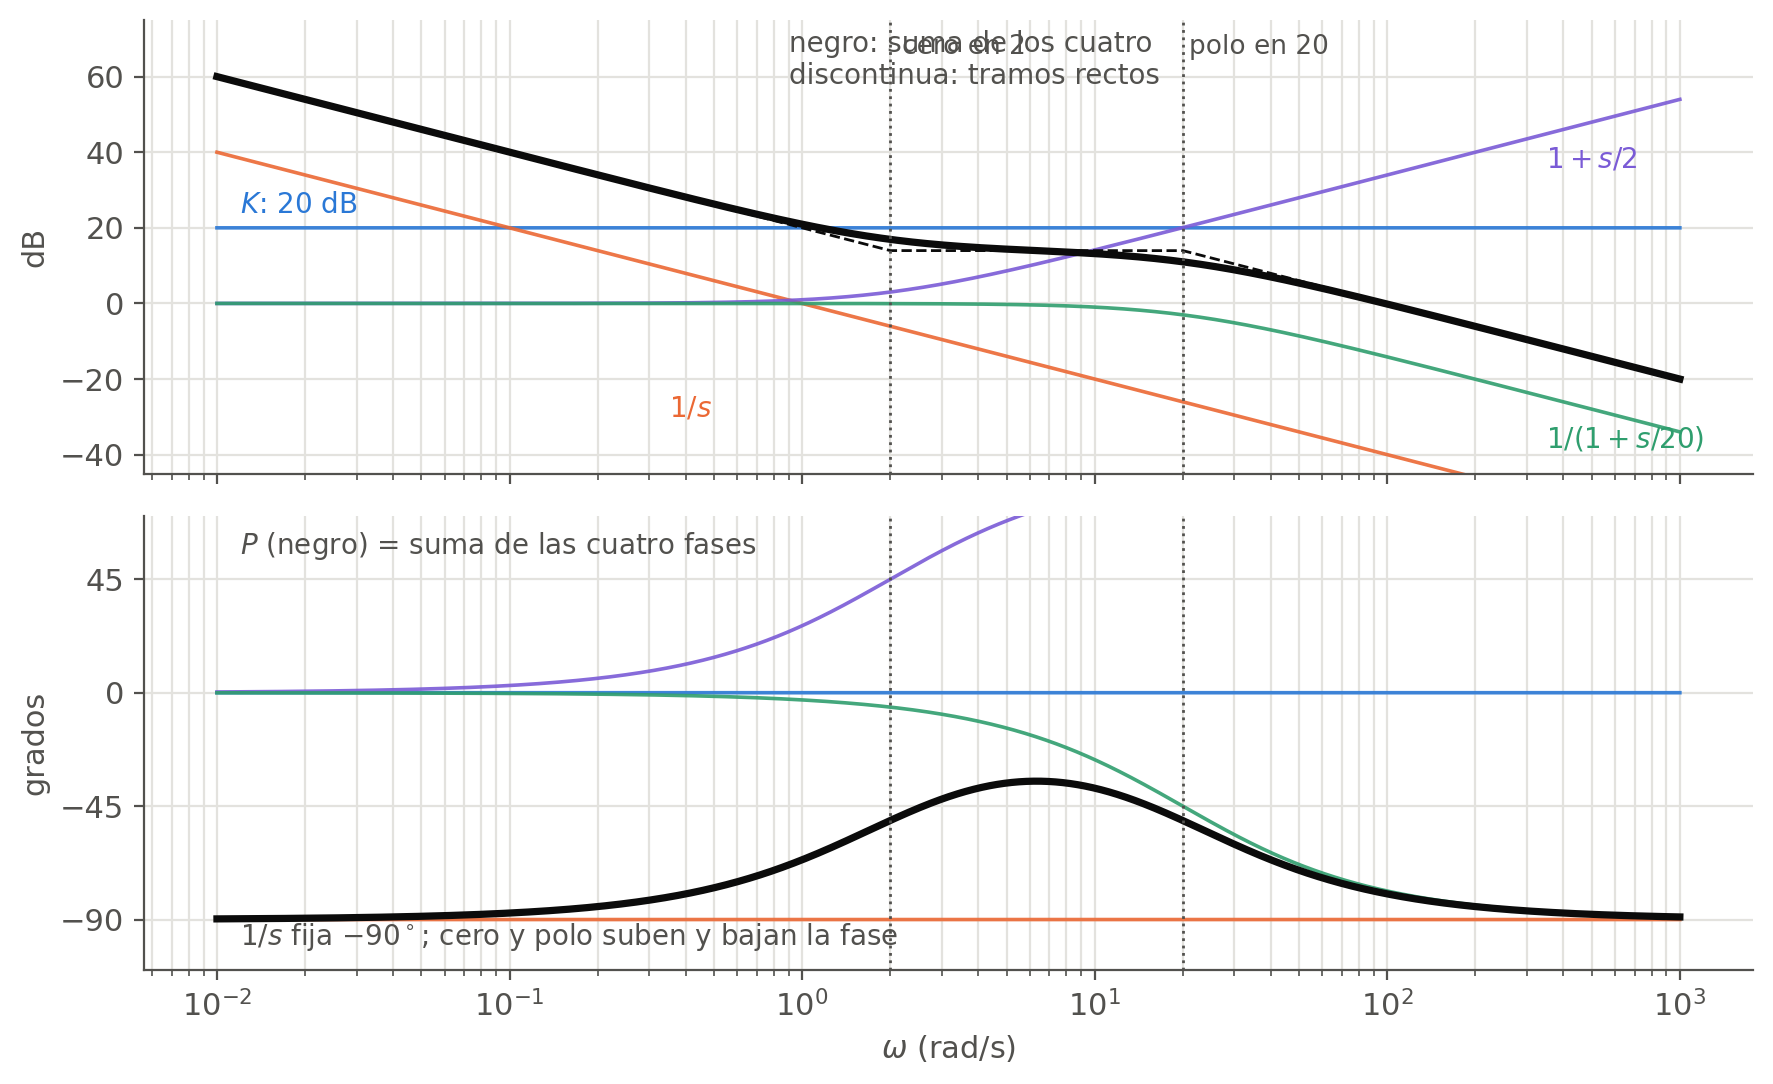
\includegraphics[width=\textwidth]{fig/construccion.png}
  \end{column}
  \end{columns}
\end{frame}

\begin{frame}{Un retardo puro: magnitud intacta, fase que se pierde}
  \footnotesize
  \begin{columns}[T]
  \begin{column}{0.5\textwidth}
    Un retardo de $T$ segundos es $e^{-sT}$, y en $s=j\omega$:
    \[ e^{-j\omega T}=1\angle(-\omega T) \]
    \begin{itemize}
      \item Módulo $1$: \textbf{0 dB siempre}.
      \item Fase $-\omega T$ rad $=-\omega T\cdot\frac{180}{\pi}$ grados: crece \emph{linealmente} con $\omega$.
    \end{itemize}
    \begin{block}{Es el paso 3 de nuevo}
      $\varphi=\omega\,\Delta t$: a mayor $\omega$, los mismos segundos son más grados. Con $T=0.1$ s: $-57.3^\circ$ a $\omega=10$ y $-573^\circ$ a $\omega=100$.
    \end{block}
    \begin{alertblock}{Por qué importa}
      Se come fase sin límite. En el Nichols será un desplazamiento horizontal.
    \end{alertblock}
  \end{column}
  \begin{column}{0.48\textwidth}
    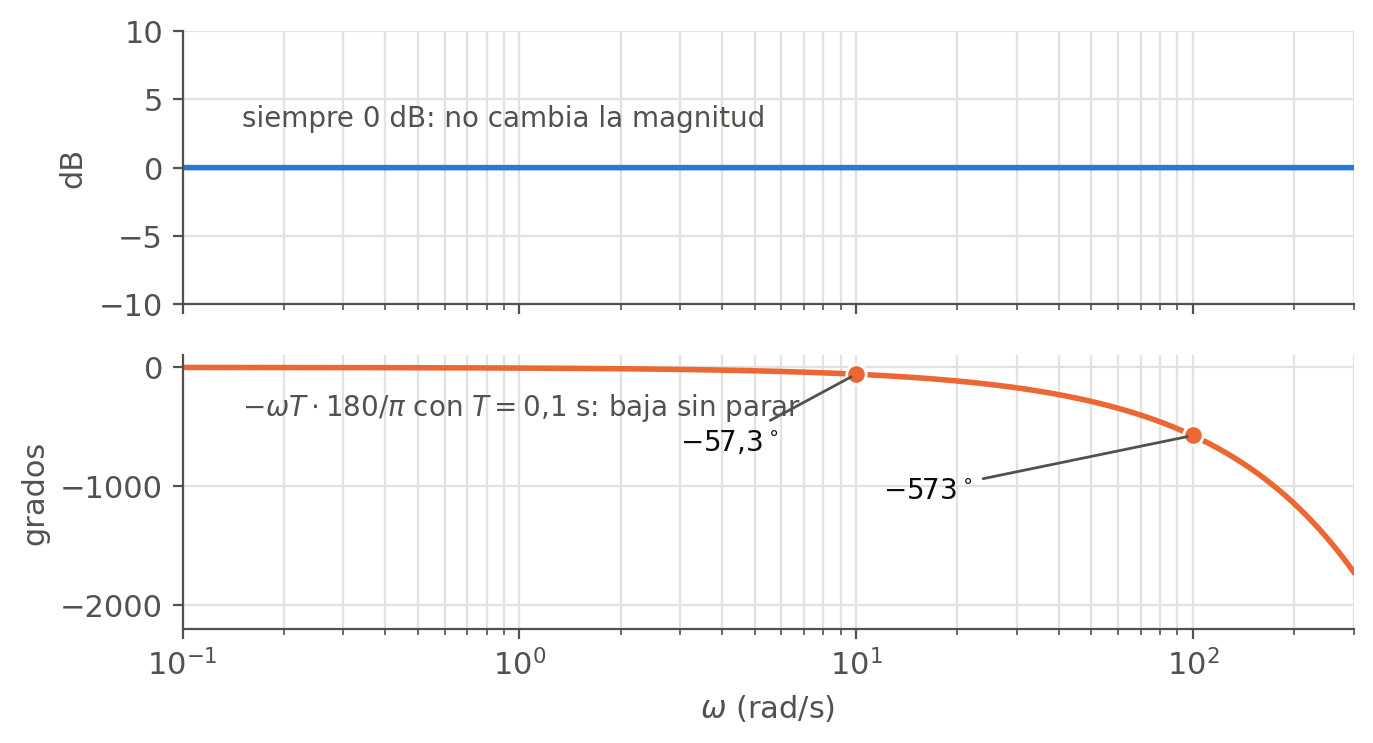
\includegraphics[width=\textwidth]{fig/retardo.png}
  \end{column}
  \end{columns}
\end{frame}

\begin{frame}{Ejercicio}
  \small
  Sea $P(s)=\dfrac{40\,(s+1)}{s\,(s+10)}$.
  \begin{enumerate}
    \item Escríbela en forma normalizada e identifica sus factores.
    \item Dibuja a mano las pendientes de la magnitud: ¿qué pendiente hay antes de $\omega=1$, entre 1 y 10, y después de 10?
    \item Calcula \textbf{exactamente} $|P(j1)|$ en dB y $\angle P(j1)$.
  \end{enumerate}
  \begin{block}{Pista}
    En el apartado 3 no hace falta dibujar: usa la suma de dB y de fases de los factores en $\omega=1$.
  \end{block}
  \textcolor{gray}{La solución está en el apéndice.}
\end{frame}

\begin{frame}{Resumen}
  \small
  \begin{itemize}
    \item $20\log_{10}|P|$: $\times10\Rightarrow+20$ dB, $\times2\Rightarrow+6$ dB, $0$ dB $\Leftrightarrow|P|=1$.
    \item Producto de factores $\Rightarrow$ \textbf{suma} en dB y suma de fases.
    \item Cuatro bloques: ganancia, integrador, polo, cero. Cada esquina cambia la pendiente en $\pm20$ dB/dec.
    \item Un retardo no toca la magnitud y resta fase $\omega T$.
    \item Siguiente paso: cerrar el lazo. Veremos qué hace $L(j\omega)$ con la salida: $T=\frac{L}{1+L}$.
  \end{itemize}
\end{frame}

\appendix
\begin{frame}\centering\Large Apéndice\end{frame}

\begin{frame}{Solución del ejercicio $P(s)=\dfrac{40(s+1)}{s(s+10)}$}
  \footnotesize
  \begin{columns}[T]
  \begin{column}{0.52\textwidth}
    \textbf{1.} $\dfrac{40\cdot1\,(1+s)}{s\cdot10\,(1+s/10)}=\dfrac{4\,(1+s)}{s\,(1+s/10)}$: $K=4$ (12.04 dB), $1/s$, cero en 1, polo en 10.\\[3pt]
    \textbf{2.} Antes de 1: $-20$ dB/dec; entre 1 y 10: $0$; después de 10: $-20$ dB/dec.\\[3pt]
    \textbf{3.} En $s=j$:
    \[ P(j)=\frac{4(1+j)}{j\,(1+0.1j)} \]
    Módulo: $\dfrac{4\cdot1.4142}{1\cdot1.0050}=5.629\Rightarrow\boxed{15.01\text{ dB}}$.\\
    Fase: $45^\circ-90^\circ-5.71^\circ=\boxed{-50.71^\circ}$.
  \end{column}
  \begin{column}{0.46\textwidth}
    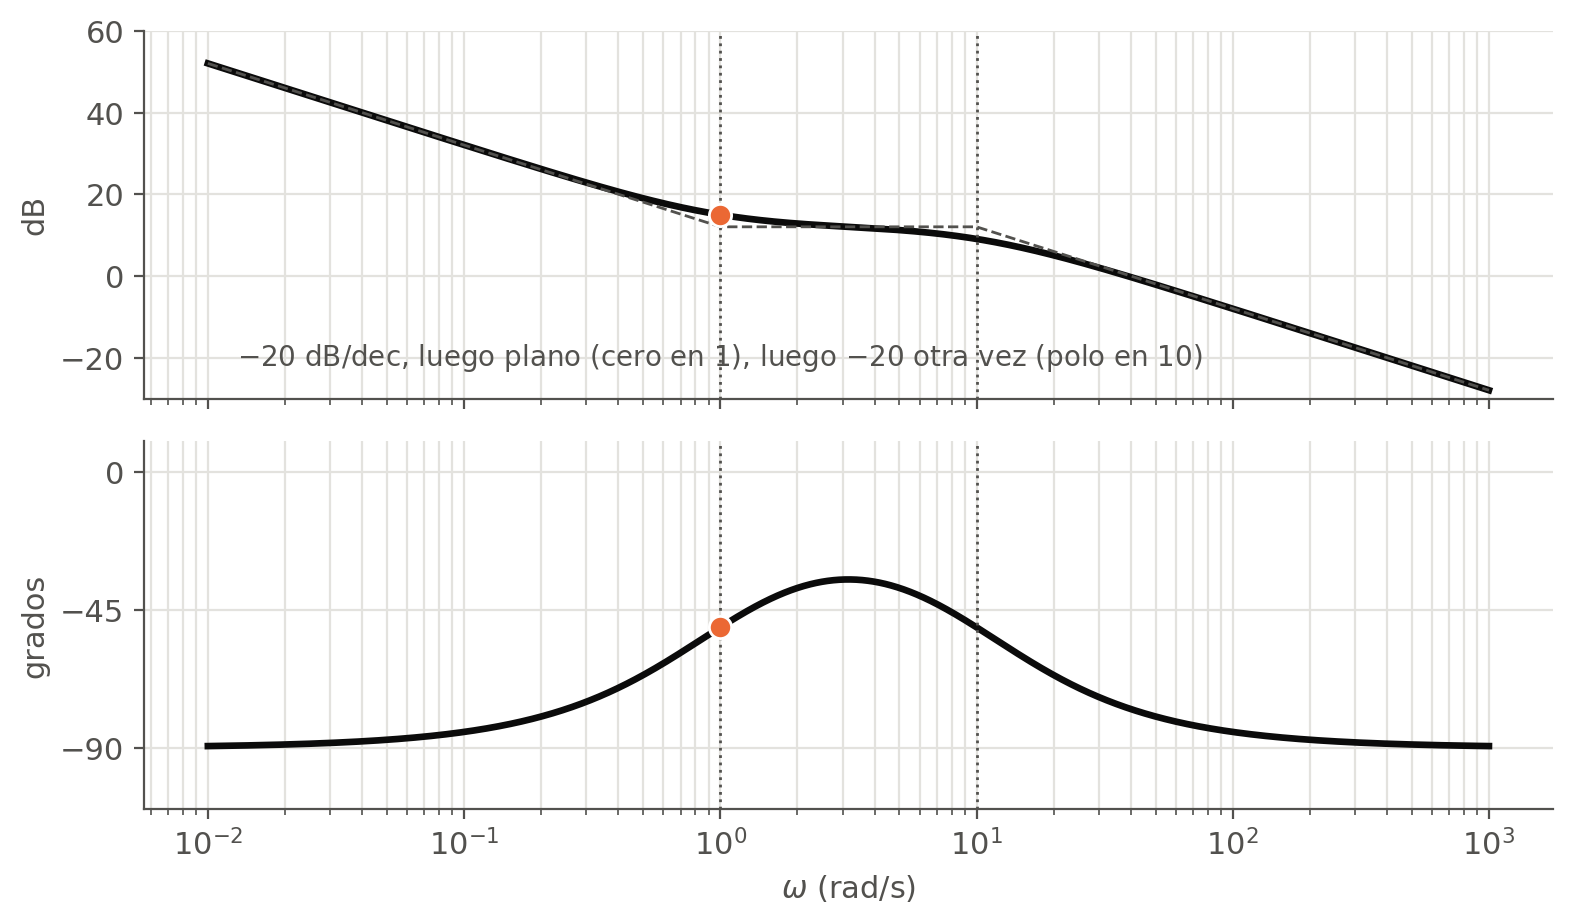
\includegraphics[width=\textwidth]{fig/solucion.png}
  \end{column}
  \end{columns}
\end{frame}
\end{document}
